\documentclass{beamer}

\usepackage[utf8]{inputenc}
\usepackage[cache=false]{minted}

\usetheme{Madrid}
\AtBeginSection[]
{
  \begin{frame}
    \frametitle{Contents}
    \tableofcontents[currentsection]
  \end{frame}
}
%--------------------------------------------

\title[Laziness in GHC Haskell]
{Laziness in GHC Haskell}

\subtitle{The features and principles}

\author[chip]
{Presented by chip}

\institute[ZJU]
{
  ZJU Lambda\\
  From here to World
}

\date[ZJU-Lambda 2019]
{ZJU-Lambda Conference, May 2019}

\logo{
\includegraphics[height=1.5cm]{./pic/haskell-logo.png}}

\begin{document}
\frame{\titlepage}


\section{Some examples}
%--------------------------------------------

\begin{frame}
\frametitle{Example 1: No evaluation}

\inputminted{haskell}{src/no-evaluation.hs}
\par\noindent\rule{0.6\textwidth}{1.0pt}
\newline\newline
Well, it prints \mintinline{haskell}{0}

\end{frame}

%--------------------------------------------

\begin{frame}
\frametitle{Example 2: Evaluate to WHNF}

\inputminted{haskell}{src/evaluate-to-WHNF.hs}
\par\noindent\rule{0.6\textwidth}{1.0pt}
\newline\newline
It prints \mintinline{haskell}{2} !
\newline
What happened here?

\end{frame}

%--------------------------------------------

\begin{frame}
\frametitle{Example 2: Evaluate to WHNF}
The actual evaluating process:
\newline
\inputminted{haskell}{src/length'-procedure.hs}

\begin{block}{Concept}
In WHNF, we only evaluate the outermost constructor
\end{block}
\end{frame}


\section{Thunk? What's it?}
%--------------------------------------------

\begin{frame}
\frametitle{The Haskell Heap}
\begin{center}
    The Haskell heap is a rather strange place.
\end{center}
\begin{figure}[hbt!]
    \centering
    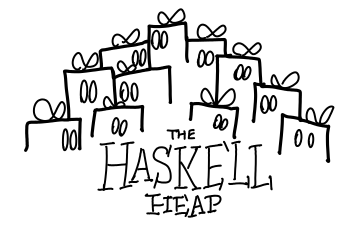
\includegraphics[height=0.5\textheight]{./pic/haskell-heap.png}
\end{figure}
\end{frame}

%--------------------------------------------

\begin{frame}
\frametitle{Thunk}
Every item is wrapped up nicely in a box:
\newline
The Haskell heap is a heap of \textit{presents} (thunks).
\begin{figure}[hbt!]
    \centering
    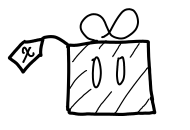
\includegraphics[height=0.5\textheight]{./pic/thunk.png}
\end{figure}
\end{frame}

%--------------------------------------------

\begin{frame}
\frametitle{Present}
When you actually want what’s inside the present, you \textit{open it up} (evaluate it).
\newline
\begin{figure}[hbt!]
    \centering
    
\includegraphics[height=0.5\textheight]{./pic/thunk-nullary.png}
\end{figure}
\end{frame}

%--------------------------------------------

\begin{frame}
\frametitle{Gift card}
Sometimes you open a present, you get a \textit{gift card} (data constructor).\newline
Gift cards have two traits.\newline
\begin{itemize}
    \item A name. (the \textbf{Just} gift card or \textbf{Right} gift card)\newline
    \item And they tell you where the rest of your presents are.\newline
\end{itemize}
There might be more than one (the tuple gift card), if you’re a lucky duck!
\begin{figure}[hbt!]
    \centering
    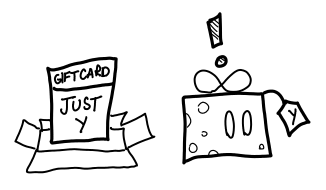
\includegraphics[height=0.4\textheight]{./pic/thunk-constructor.png}
\end{figure}
\end{frame}


\end{document}